%% Based on a TeXnicCenter-Template by Tino Weinkauf.
%%%%%%%%%%%%%%%%%%%%%%%%%%%%%%%%%%%%%%%%%%%%%%%%%%%%%%%%%%%%%

%%%%%%%%%%%%%%%%%%%%%%%%%%%%%%%%%%%%%%%%%%%%%%%%%%%%%%%%%%%%%
%% HEADER
%%%%%%%%%%%%%%%%%%%%%%%%%%%%%%%%%%%%%%%%%%%%%%%%%%%%%%%%%%%%%
\documentclass[a4paper,12pt]{report}
% Alternative Options:
%	Paper Size: a4paper / a5paper / b5paper / letterpaper / legalpaper / executivepaper
% Duplex: oneside / twoside
% Base Font Size: 10pt / 11pt / 12pt


%% Language %%%%%%%%%%%%%%%%%%%%%%%%%%%%%%%%%%%%%%%%%%%%%%%%%
\usepackage[USenglish]{babel} %francais, polish, spanish, ...
\usepackage[utf8x]{inputenc}
%\usepackage[ansinew]{inputenc}

\usepackage{lmodern} %Type1-font for non-english texts and characters


%% Packages for Graphics & Figures %%%%%%%%%%%%%%%%%%%%%%%%%%
\usepackage{graphicx} %%For loading graphic files
%\usepackage{subfig} %%Subfigures inside a figure
%\usepackage{pst-all} %%PSTricks - not useable with pdfLaTeX



%% Math Packages %%%%%%%%%%%%%%%%%%%%%%%%%%%%%%%%%%%%%%%%%%%%
\usepackage{amsmath}
\usepackage{amsthm}
\usepackage{amsfonts}
\usepackage{xurl}

%% Other Packages %%%%%%%%%%%%%%%%%%%%%%%%%%%%%%%%%%%%%%%%%%%
%\usepackage{a4wide} %%Smaller margins = more text per page.
%\usepackage{fancyhdr} %%Fancy headings
%\usepackage{longtable} %%For tables, that exceed one page
\usepackage[dvipsnames]{xcolor}
\usepackage{subcaption}
\usepackage[export]{adjustbox}
\usepackage[a4paper, margin=2cm]{geometry}
\usepackage{float}
\usepackage{tikz,siunitx}	


\usepackage{listings}
%%remove the paragraph indent for the whole document
\setlength\parindent{0pt}

%%%%%%%%%%%%%%%%%%%%%%%%%%%%%%%%%%%%%%%%%%%%%%%%%%%%%%%%%%%%%
%% DOCUMENT
%%%%%%%%%%%%%%%%%%%%%%%%%%%%%%%%%%%%%%%%%%%%%%%%%%%%%%%%%%%%%
\begin{document}

\pagestyle{empty} %No headings for the first pages.


%% Title Page %%%%%%%%%%%%%%%%%%%%%%%%%%%%%%%%%%%%%%%%%%%%%%%
%% ==> Write your text here or include other files.

%% The simple version:
%\title{Title of this document}
%\author{Firstname Lastname}
%%\date{} %%If commented, the current date is used.
%\maketitle

\begin{titlepage}

		\begin{figure}[t]

			\begin{subfigure}{0.5\textwidth}
			
\includegraphics[width=0.9\linewidth, left]{image/serval-logo-2-black.png}
			\end{subfigure}
		\end{figure}

    \begin{center}
        \vspace*{2cm}
				
        \Huge
        \textbf{\textcolor{BlueViolet}{Serval PROJECT}}
        
        \vspace{0.5cm}
        \LARGE
				\textcolor{blue}{Documentation for serval test network}
				\noindent\color{BlueViolet}\rule{\textwidth}{2pt}
		\end{center}        
		\vspace{1.5cm}
		
		\vfill
		
		\noindent\textcolor{Blue}{
		\large \noindent Author: Stephane IMBERT\\
		Exchange student at Flinders University\\
		Project supervisor: Dr Paul Gardner-Stephen
		}
		
		\vspace{2cm}	
		
		\noindent\large Submitted to the School of Computer Science, Engineering, and Mathematics in the Faculty 
of Science and Engineering in partial fulfilment of the requirements for the degree of Master of Computer Science at Flinders University –
 Adelaide Australia.
		
		\vspace{1.5cm}
		\noindent\large
		Flinders University at Tonsley\\
		1284 South Road\\
		Clovely Park SA 5042
\end{titlepage}




%% Inhaltsverzeichnis %%%%%%%%%%%%%%%%%%%%%%%%%%%%%%%%%%%%%%%
\tableofcontents %Table of contents
\cleardoublepage %The first chapter should start on an odd page.

\pagestyle{plain} %Now display headings: headings / fancy / ...



\chapter{general presentation of the test network}


\section{Goals}

The foal of the project was to build a test network for the Mesh Extenders. 
We want to have Mesh Extenders at different places in a building. The Mesh extenders are communicating together using UHF (they need to far enough from each other or have their Wi-Fi range limited by any way). Each Mesh extender is connected to a phone by Wi-Fi.

The test network is built around this basic setup. We want to be able to remotely supervise and control each site.
To do that we are going to built a test network with:
\begin{itemize}
	\item a software part using c programs
	\item a hardware part using small linux routers
\end{itemize}



\section{Components}

As previously said, the test network is made of a software and a hardware part.

\subsection{Hardware components}

First, for this test network, we will obviously need Mesh Extenders:
\begin{figure}[H]
\begin{center}
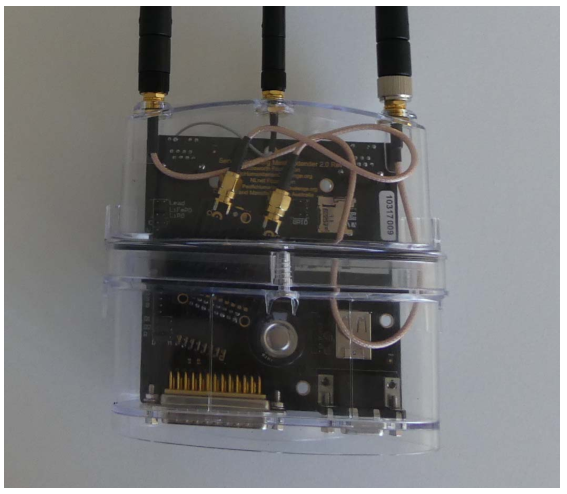
\includegraphics[width=8cm]{image/meshextender.png}%
\caption{Mesh Extender}%
\label{figure:ME}%-
\end{center}
\end{figure}


In this project we are also using small linux routers to built the network we will use to supervise the Mesh Extenders.

The small router we have chose to use are: the GL-AR150 and GL-AR750.

\begin{figure}[H]
\centering
\begin{subfigure}{.5\textwidth}
  \centering
	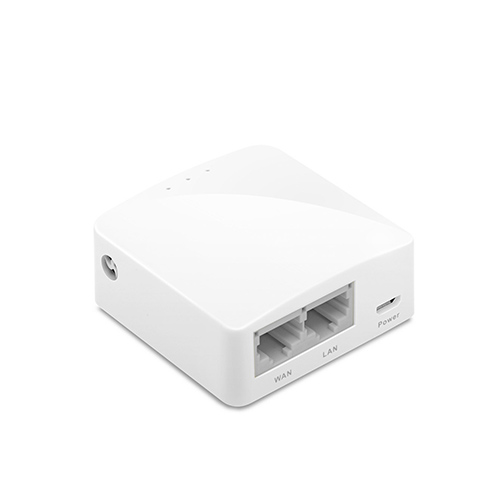
\includegraphics[width=8cm]{image/AR150.jpg}%
	\caption{GL-AR150}%
	\label{figure:AR150}%-
\end{subfigure}%
\begin{subfigure}{.5\textwidth}
  \centering
  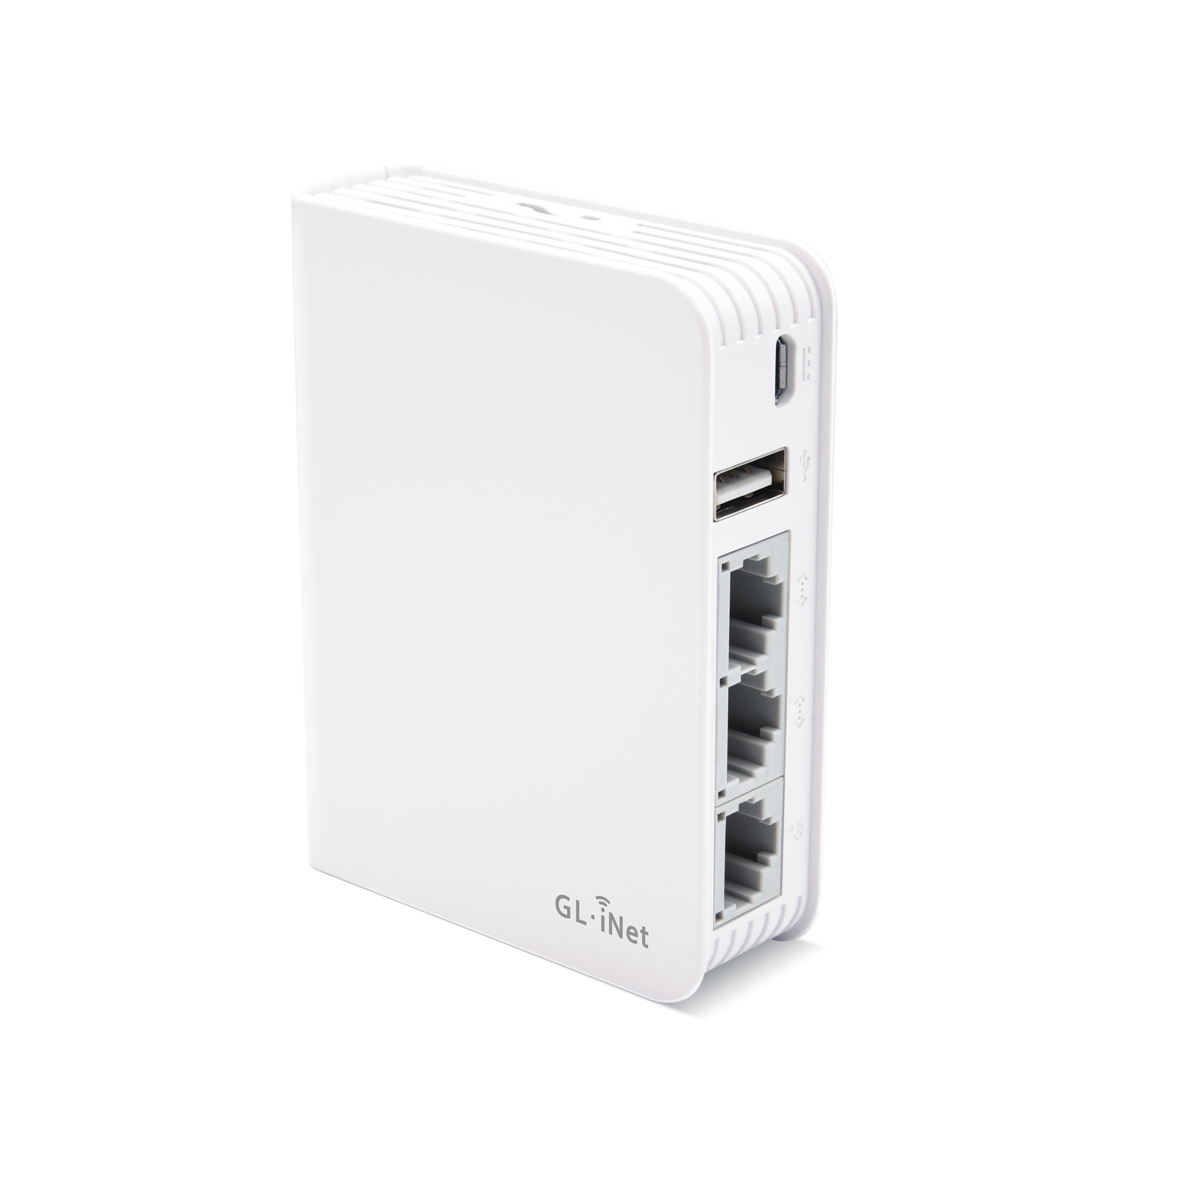
\includegraphics[width=8cm]{image/AR750.jpg}%
	\caption{GL-AR750}%
	\label{figure:AR750}%-
\end{subfigure}
\caption{Routers used for the testbed}
\label{fig:routers}
\end{figure}


These two routers are great for the test network. Indeed, they are small, affordable and we have a lot of freedom since their OS is based on a Linux kernel (the OS used for the Mesh extenders can also be put inside these routers).
The only issue we can have is the fact they do not have a lot of USB port and also no UHF radio. Therefore we need other devices:
\begin{figure}[H]
\centering
\begin{subfigure}{.5\textwidth}
  \centering
	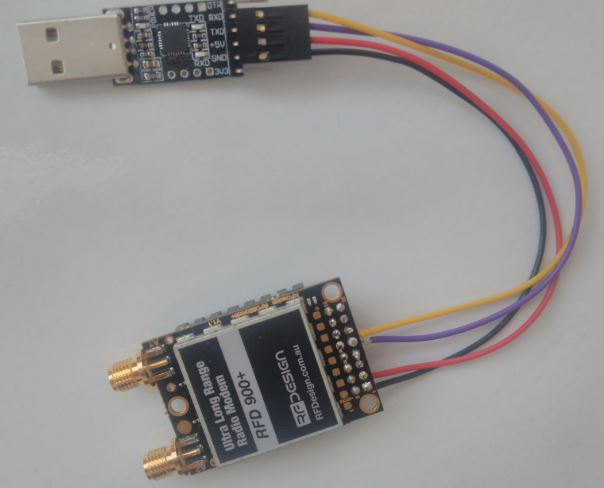
\includegraphics[width=8cm]{image/rfd900.jpg}%
	\caption{RFD900 with a serial to USB adapter}%
	\label{figure:RFD900}%-
\end{subfigure}%
\begin{subfigure}{.5\textwidth}
  \centering
  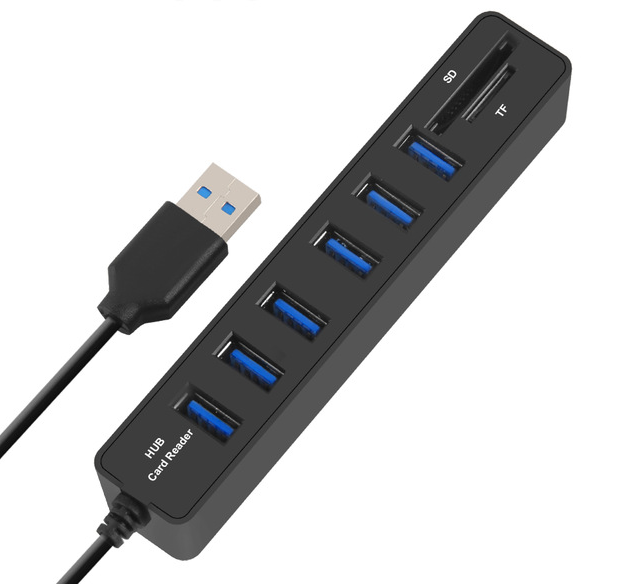
\includegraphics[width=8cm]{image/usbhub.jpg}%
	\caption{USB hub}%
	\label{figure:UsbHub}%-
\end{subfigure}
\caption{Other devices needed}
\label{fig:devices}
\end{figure}

To monitor the UHF packets of the Mesh Extenders, we need a RFD900+. Since the RFD900+ has a serial interface (pins), we need to create an adapter to plug it using USB.
We are using a USB hub to increase the number of USB ports on the router.

We now have all the needed hardware.



\subsection{software}

In this project, we are going to use c programs to remotely supervise the Mesh Extenders.
C language was chosen because:
\begin{itemize}
	\item it is a light and efficient language (which is great since our routers don't have a lot of power or memory)
	\item In the Serval project most of the coding was made in c. We can easily integrate other part of the serval project inside the test network.
\end{itemize}


I have decide to create a TCP client-server system composed of 3 files:
\begin{itemize}
	\item server.c which will be on the small routers
	\item client\_shell.c and client.c which will be on the computer used to supervise
\end{itemize}

I will explain what each file does in the next section.


A TCP client-server was not the only solution. However, I still opted for it because:
\begin{itemize}
	\item I was more used to code TCP server and client than other solutions. Therefore I will be faster using this solution.
	\item The libraries for TCP are quite old and should work on most devices.
\end{itemize}



\section{Big picture}

We will now take a look at how the network and software work.


\subsection{Big picture of the network}
%BIG  picture of the network





\subsection{Big picture of the software}



The software part corresponds to the communication between a few programs:
\begin{itemize}
	\item the client\_shell and the client
	\item the client and the server
	\item the server and the RFD900+
\end{itemize}

For the communication between the server and the RFD900+, we use the driver in c developed by Paul. This part use the code of the lbard git repository.


\subsubsection{client to server communication}

The communication between the client and the server is very basic. Most of the time the client is only receiving packet from the server and display them on the computer.

But the client can also send a few message to the server. This messages allow the client to close the communication with the server. Later they will also allow the client to change what is supervised.

\begin{figure}[H]
\begin{center}
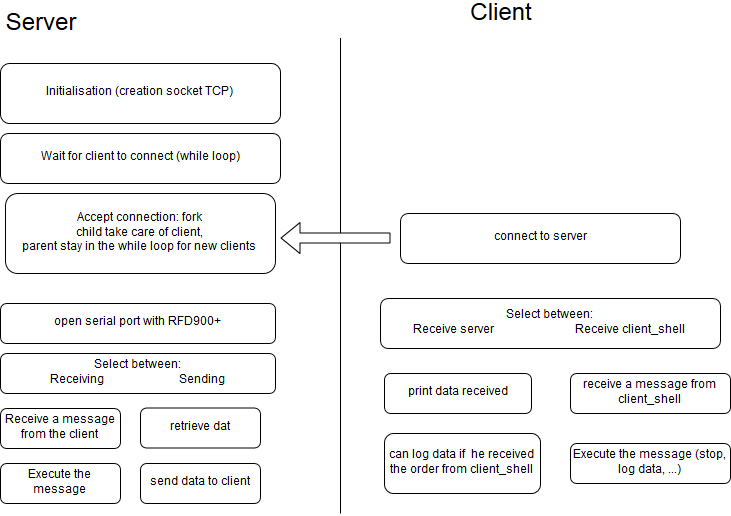
\includegraphics[width=\textwidth]{image/clientServer.png}%
\caption{Client and server communication}%
\label{figure:CS}%-
\end{center}
\end{figure}





\subsubsection{client\_shell and client interactions}

The client\_shell is a shell-like interface that gives access to all the available functionalities.
It can:
\begin{itemize}
	\item find the available servers using a file containing the hostnames of servers
	\item launch a client
	\item communicate with the client to send different orders such as
		\subitem "`STOP"' to close the connection
		\subitem "`LOG Filename"' to start logging the data
  \item keep a list of all the current client created
	\end{itemize}




\begin{figure}[H]
\begin{center}
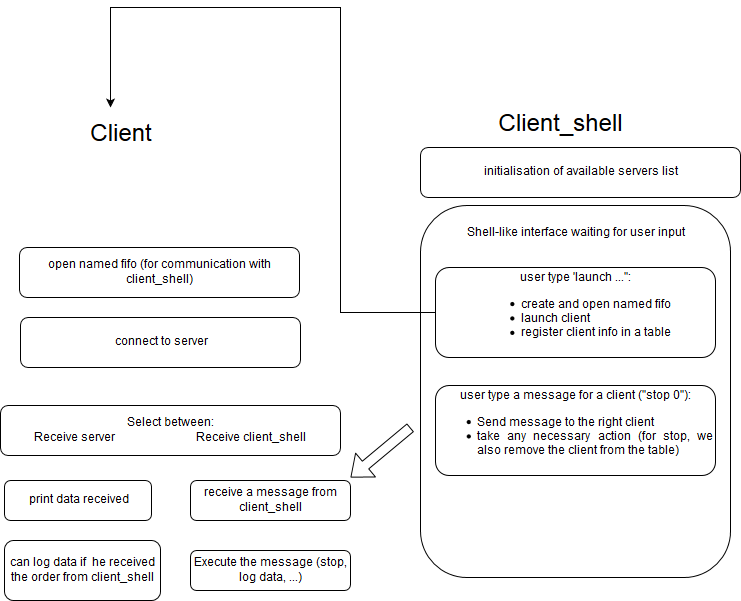
\includegraphics[width=\textwidth]{image/clientshellClient.png}%
\caption{Client and Client\_shell interaction}%
\label{figure:CSC}%-
\end{center}
\end{figure}



\chapter{Install}


\section{Basic requirements}


To install this network, you will need a few devices.
First you will need a computer with a linux OS (the development of the project was done on Ubuntu). But you also need a few devices:
\begin{itemize}
	\item routers that support openwrt (I used GL-AR150 and GL-AR750)
	\item RFD900+ with serial to usb adaptor
\end{itemize}

Here is a list of all the package you need on your Linux machine:
\begin{itemize}
	\item gcc 
	\item binutils
	\item bzip2
	\item flex
	\item python
	\item perl
	\item make
	\item find
	\item grep
	\item diff
	\item unzip
	\item gawk
	\item getopt
	\item subversion
	\item libz-dev
	\item libc headers
\end{itemize}



\section{Network setup}


For this part, i will suppose you are using openwrt or Lede routers that support wireless communication.

First let's start by looking at the result we want. 
We have many remote sites and 1 main site. The main site is a Wi-Fi access to all the remote sites and it will be the main part of the configuration.

For this site I used GL-AR750. 
We will have a main router and a "`slave"' router.
The main router will have a DHCP server and he will therefore give the addresses to all the devices.

The slave router will connect to the main router and act as a Wi-Fi bridge. 
The GL-AR750 does not allow us to "`physically"' bridge our local network (Wi-Fi + ethernet ports) and the connection with the main router. That's why we are going to use a packet called relayd that will allow us to simulate that bridge.

So the general steps are:
\begin{itemize}
	\item Configure the main router by:
		\subitem creating a Wi-Fi LAN 
		\subitem configuring fixed ip addresses for the small remote routers
	\item Configuring the slave router by:
		\subitem installing relayd
\end{itemize} 

We want to create a network like the one below:
\begin{figure}[H]
\begin{center}
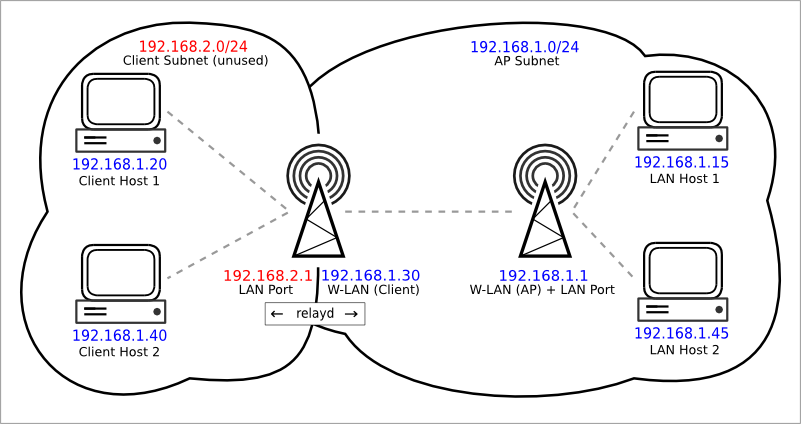
\includegraphics[width=\columnwidth]{image/802-11-routed-relay.png}%
\caption{Bridge network using relayd (source:https://wiki.openwrt.org/doc/recipes/relayclient)}%
\label{figure:interface3}%-
\end{center}
\end{figure}


\subsection{Configuration of the main router}

All the configuration is done through the web interface at the address: http:\/\/192.168.8.1\/cgi-bin\/luci.
The IP address can change depending on the router you have. If you are using routers from GL-INET such as GL-AR750, it should be 192.168.8.1. Otherwise, you need to look at the documentation of your router.


\hfill \break \underline{\large{\textbf{Creating the Wi-Fi LAN}}}

The first we want to do is to create the Wi-Fi and setup the LAN. 
So we first go to the Network $\rightarrow$ wireless tab.
On this tab you should have two pre-configure networks (if you are using a GL-AR750).


We can remove all the networks here and we are going to create a new one. Once created, we will get the following page:
%figure
\begin{figure}[H]
\begin{center}
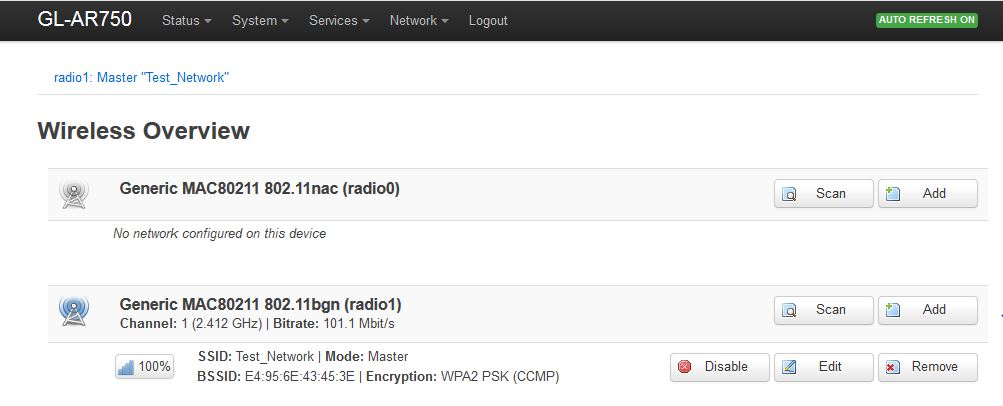
\includegraphics[width=\columnwidth]{image/wireless1.jpg}%
\caption{Wi-Fi network created}%
\label{figure:wireless1}%-
\end{center}
\end{figure}



To create this network, you click on add. It will open a new page that you need to configure as such:
%figure
\begin{figure}[H]
\begin{center}
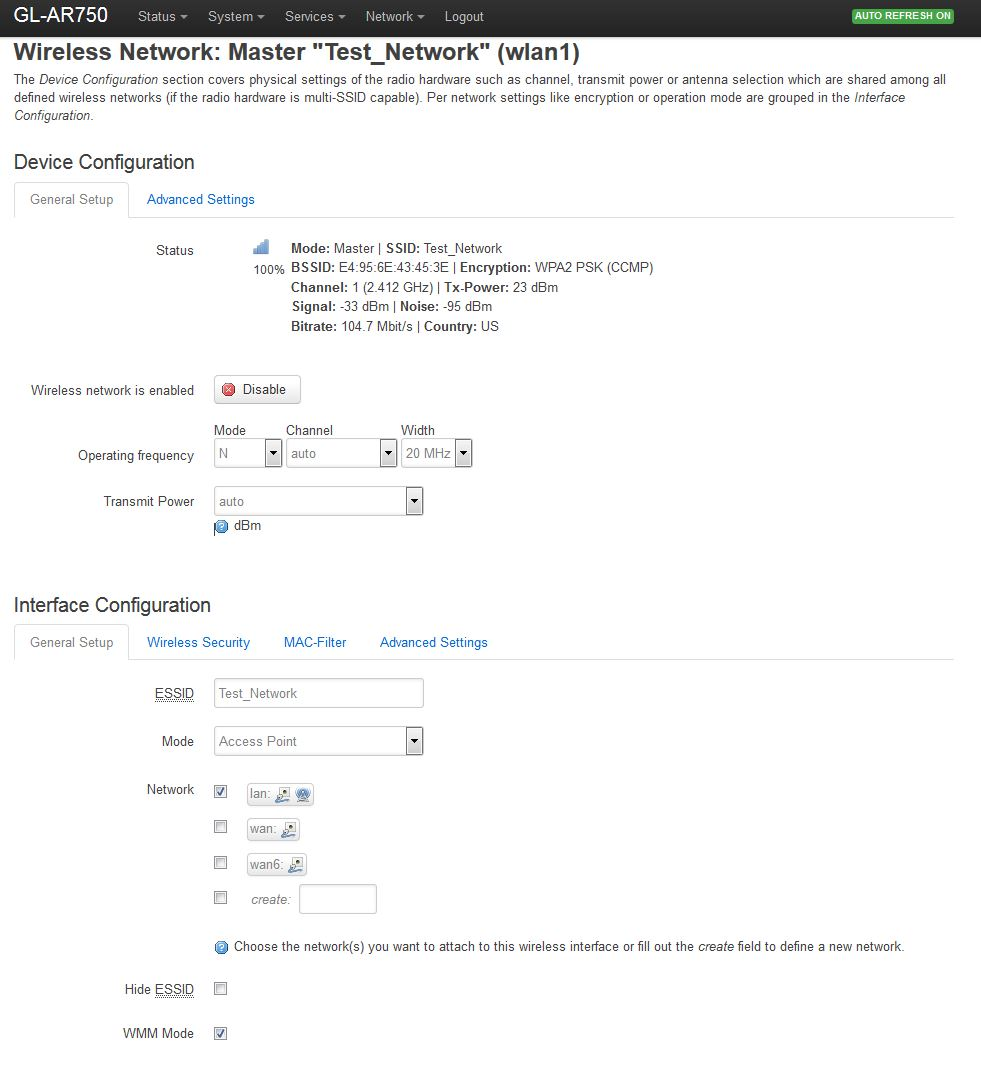
\includegraphics[width=\columnwidth]{image/wireless2.jpg}%
\caption{General configuration of the Wi-Fi network}%
\label{figure:wireless2}%-
\end{center}
\end{figure}


On the device configuration, we want the router to automatically choose the channel.
On the interface configuration, we want to:
\begin{itemize}
	\item choose an SSID
	\item choose the mode Access Point
	\item the network is lan
\end{itemize}

We now go on the wireless security tab and set it up like below:
%figure
\begin{figure}[H]
\begin{center}
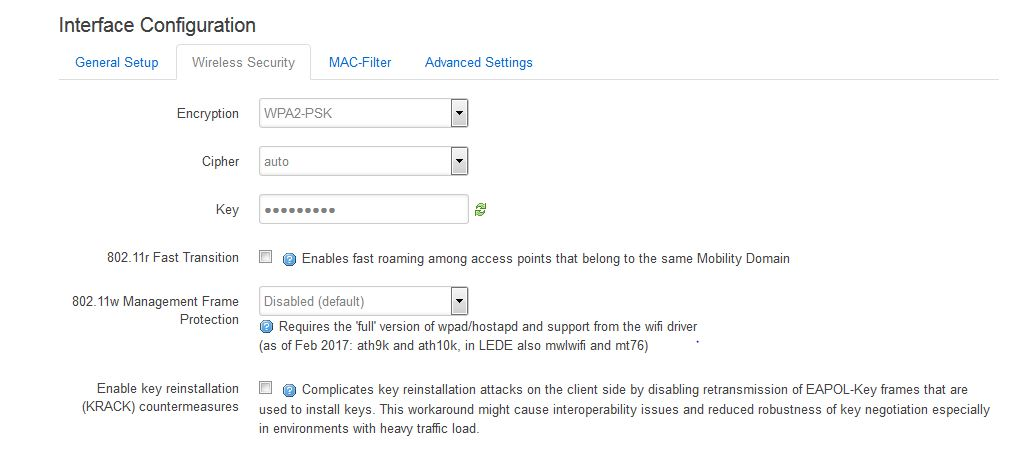
\includegraphics[width=\columnwidth]{image/wireless3.jpg}%
\caption{Security parameters}%
\label{figure:wireless3}%-
\end{center}
\end{figure}
Here we want to create

We are now done and can save the changes. We have successfully created a new Wi-Fi network. We can move on the DHCP setup.

\hfill \break \underline{\large{\textbf{Static DHCP lease}}}

For that part, we go to the Network $\rightarrow$ DHCP and DNS tab. We go at the bottom of the new page to find the section "Static Leases".
In this section, we can add static DHCP leases. We configure it like that:
%figure
\begin{figure}[H]
\begin{center}
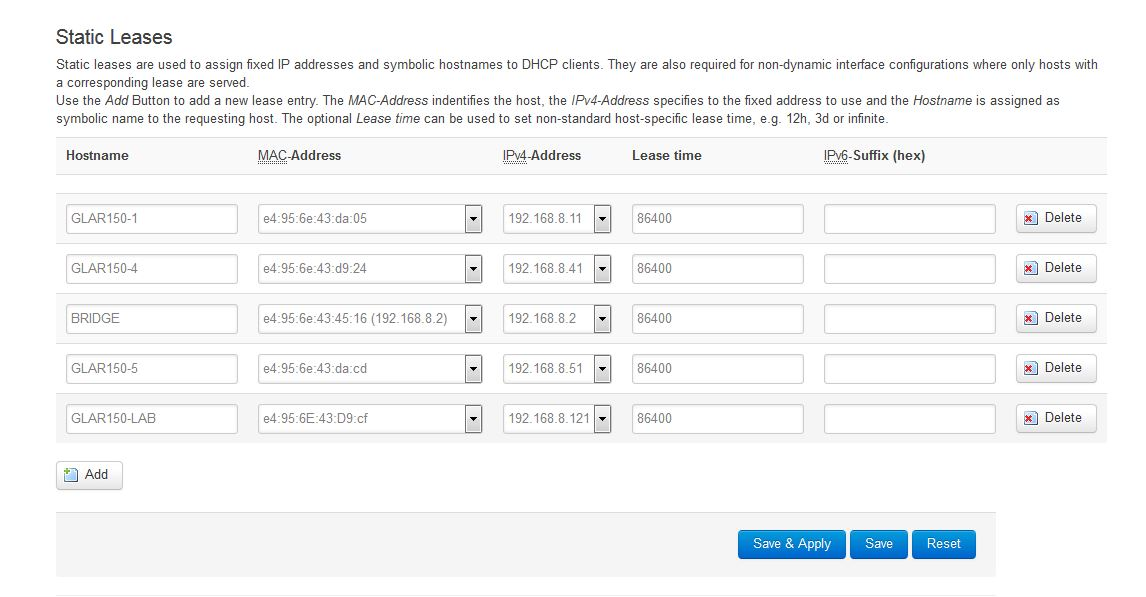
\includegraphics[width=\columnwidth]{image/DHCP1.jpg}%
\caption{DHCP static leases }%
\label{figure:DHCP1}%-
\end{center}
\end{figure}


Pressing the button add, we can manually add a static lease. Static lease work using the mac address of the device. 

\subsection{slave router configuration}

The slave router is a bit more complex to install. Indeed with a GL-AR750, by default, it is not possible to bridge a Wi-Fi Network to another Wi-Fi network. Thankfully, a linux package lets you simulate this behaviour. This package is relayd.
So we are going to install and setup relayd.

\hfill \break \underline{\large{\textbf{Installation of relayd}}}

To install relayd, we need to give the router an access to internet. To do that, you can simply plug the WLAN Ethernet interface to your internet access point or you can plug it to your computer and make your computer share its connection.

Then you connect to the router with ssh (on windows you can use putty).
We want to install two packages:
\begin{itemize}
	\item relayd
	\item luci-proto-relay
\end{itemize}

For that you can use the command:
\begin{lstlisting}
	opkg install package
\end{lstlisting}

Once the package installed we are going to set it up through the web interface. We can use this tutorial to help us:https://wiki.openwrt.org/doc/recipes/relayclient.

We can connect to the same web page as earlier (but for the slave router):http://192.168.9.1/cgi-bin/luci/
The global steps are the following:
\begin{itemize}
	\item Join the network of the main router created earlier
	\item Set up the Wi-Fi interface
	\item create the bridge interface with relayd
	\item update the LAN interface
	\item Set up the firewall
\end{itemize}

\hfill \break \underline{\textbf{Joining the network of the main router}}

The slave server is going to be a client of the main router. For that we head up to Network $\rightarrow$ wireless. We remove the existing network and we create a new one:

\begin{figure}[H]
\begin{center}
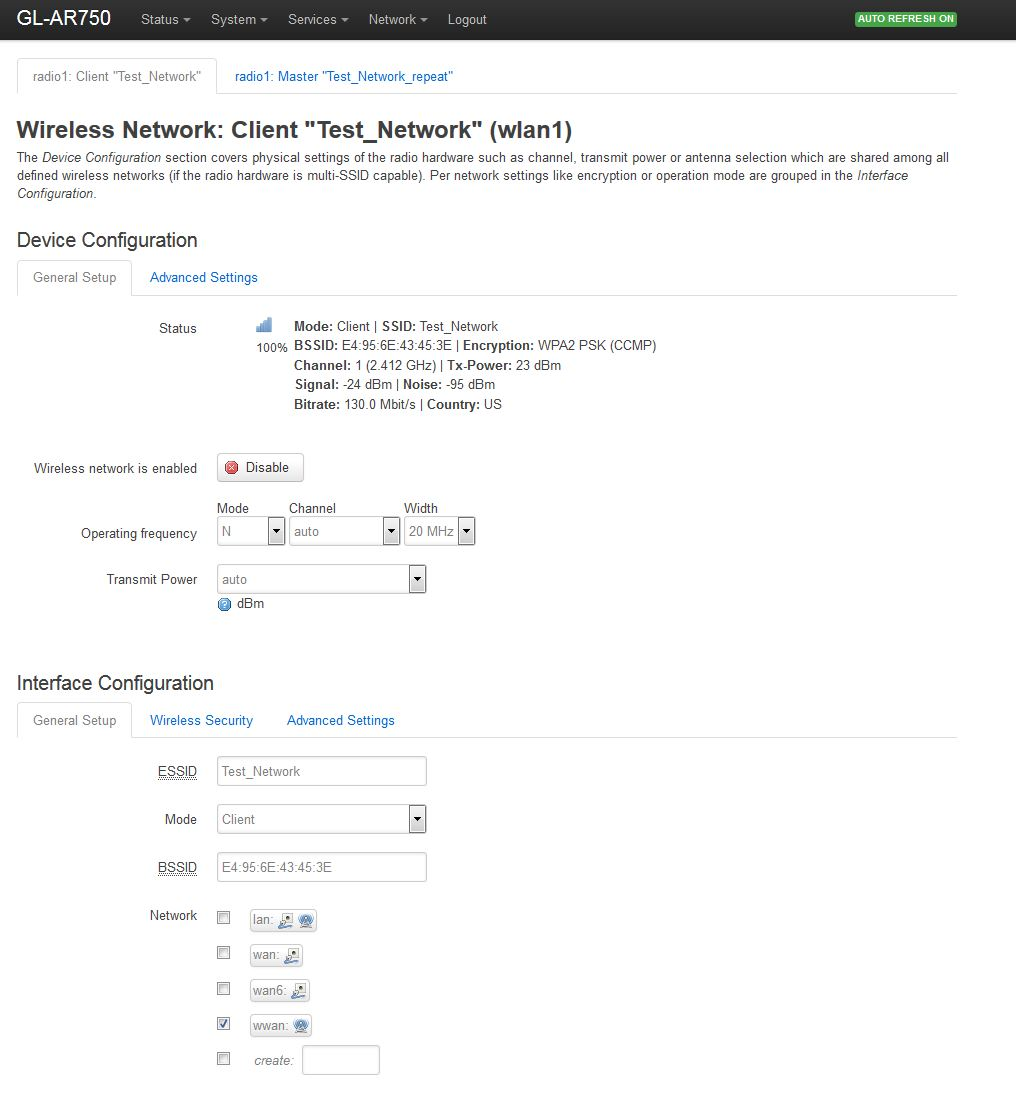
\includegraphics[width=\columnwidth]{image/wireless4.jpg}%
\caption{Joining the main router network}%
\label{figure:wireless4}%-
\end{center}
\end{figure}

We configure this network in the same way as the network on the main router. The only difference is the mode and the network. Instead of choosing access point, we choose Client. For the network, we create a new one and call it wwan (it will not exist at first, you need to enter it in the create field). We save and apply theses changes.

\hfill \break \underline{\textbf{Create a new Wi-Fi network}}

We are going to create a new Wi-Fi network. We go to the Network $\rightarrow$ interfaces and click on edit for the "WWAN" interface.
In the "General Setup" we change the protocol to "DHCP Client" (this means that the slave router will automatically get its IP address from the main router).



\hfill \break \underline{\textbf{Create the bridge interface}}

We go back to the Network $\rightarrow$ interface tab. Here, we create a new interface by clicking "Add new interface".
We set it up like that:

\begin{figure}[H]
\begin{center}
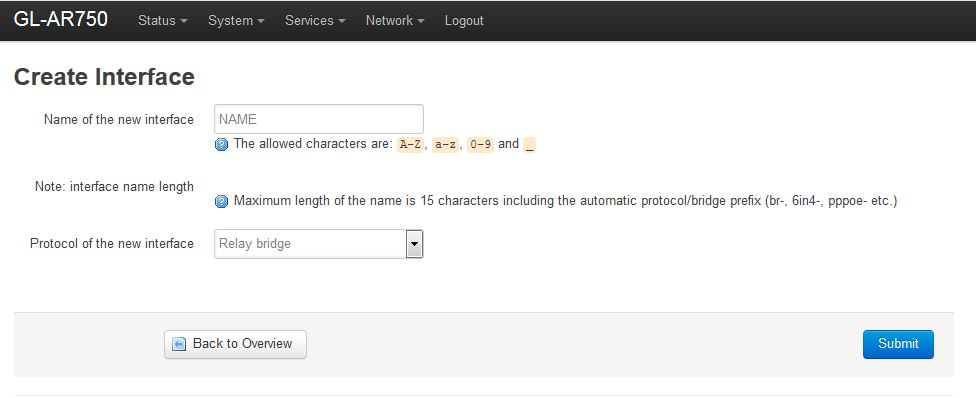
\includegraphics[width=\columnwidth]{image/interface2.jpg}%
\caption{Creation of the bridge interface}%
\label{figure:interface2}%-
\end{center}
\end{figure}

You can choose the name you want for this new interface. I personally chose REPEATER\_TEST. The important setting is protocol. We want to choose "Relay bridge". This option will only appear if we have installed the package luci-proto-relay and the package relayd.
We validate the creation by submitting it.

Now we go back to the interfaces. A new interface, bearing the name we chose, is present. We are going to edit it like the figure below:
\begin{figure}[H]
\begin{center}
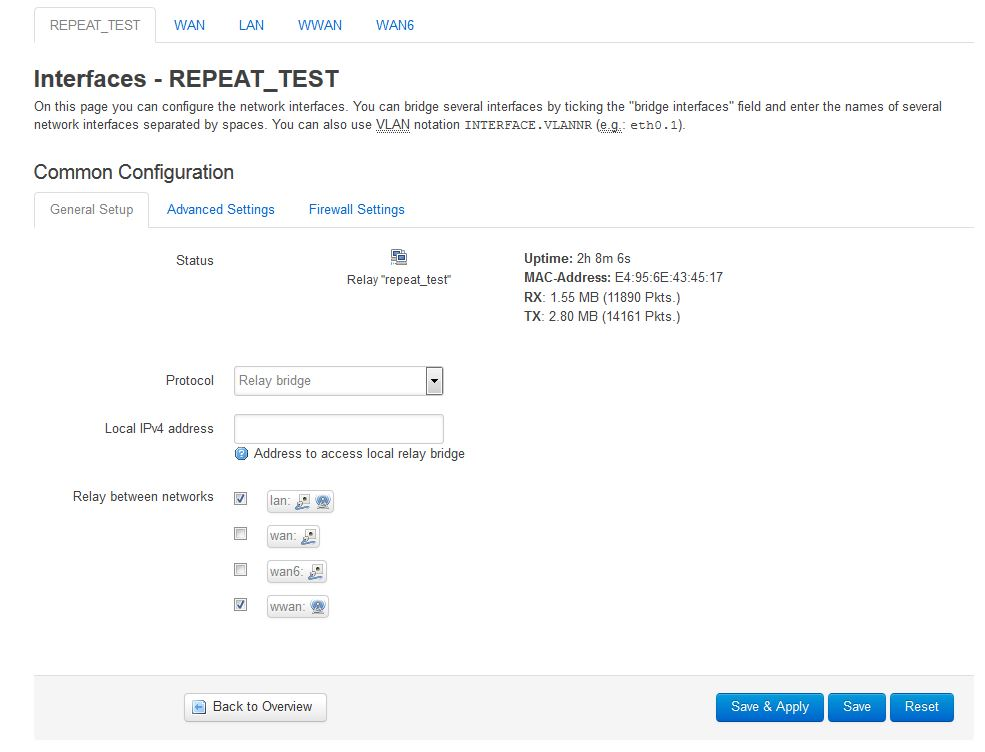
\includegraphics[width=\columnwidth]{image/interface3.jpg}%
\caption{General set up the bridge interface}%
\label{figure:interface3}%-
\end{center}
\end{figure}
Here we want to choose the network we want to bridge. We want to bridge the LAN network to the WWAN one. Therefore, every client that connect to the LAN of this router will be bridged to the WWAN network and therefore the main router.

In the "Advanced Settings", we want to make sure that "Forward DHCP traffic" is ticked (it should be ticked by default):
\begin{figure}[H]
\begin{center}
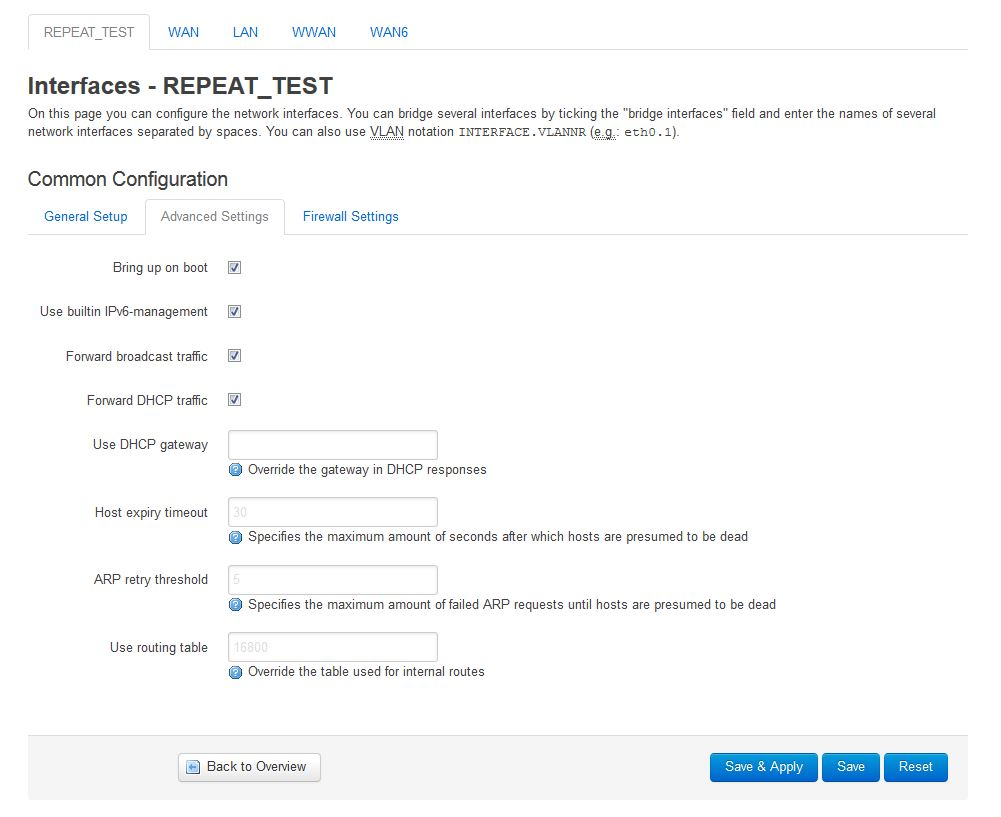
\includegraphics[width=\columnwidth]{image/interface4.jpg}%
\caption{Advanced settings of the bridge interface}%
\label{figure:interface4}%-
\end{center}
\end{figure}

We are now done with the bridge interface and we need to modify the LAN interface.



\hfill \break \underline{\textbf{Update the LAN interface}}

We go to the Network $\rightarrow$ Interfaces tab. We want to edit the LAN interface like below:
\begin{figure}[H]
\begin{center}
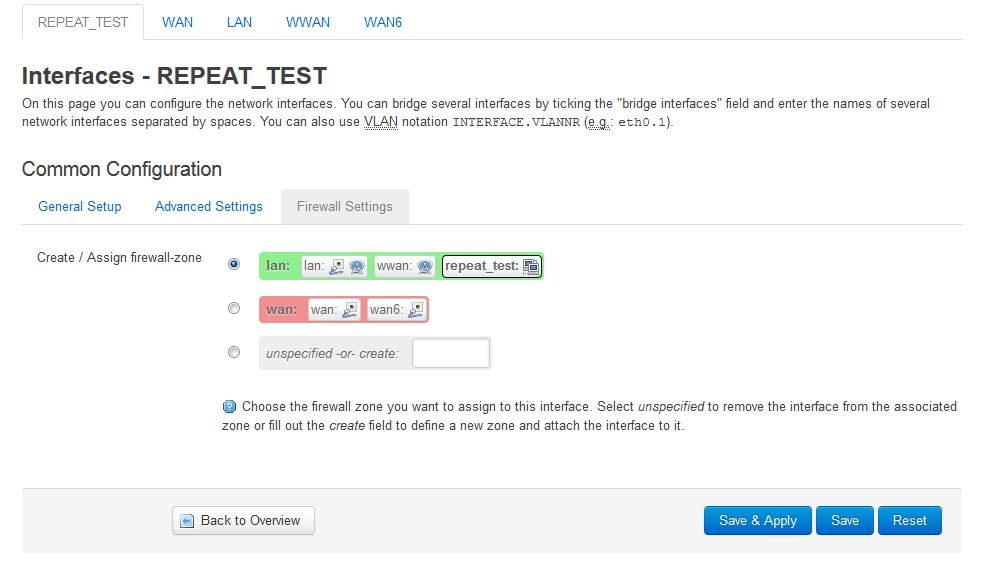
\includegraphics[width=\columnwidth]{image/interface5.jpg}%
\caption{General settings of the LAN interface}%
\label{figure:interface5}%-
\end{center}
\end{figure} 

Here we are going to use a fix address and no DHCP. We want a different address than the one used by the main router.





\hfill \break \underline{\textbf{Set up the firewall}}



\hfill \break \underline{\textbf{Set up the firewall}}


\subsection{remote router configuration}

The configuration of the remote router is quite easy. It has 2 steps:
\begin{itemize}
	\item modify the traffic rules of the router
	\item modify the configuration of the LAN interface
\end{itemize}

\section{Software installation}

The software part consist at downloading the sources files and installing them. We want to install 2 differents part:
\begin{itemize}
	\item a client part for linux
	\item a server part for openwrt
\end{itemize}

\subsection{client installation}

The client part is pretty straightforward as you just need to use the makefile by tiping:
\begin{lstlisting}[language=bash]
	###: make client
\end{lstlisting}
It will create two executable files: 
\begin{itemize}
	\item the main one is the client\_shell. It is the program the user is going to launch.
	\item the other one is the client which is used by the client\_shell to connect to the server
\end{itemize}


\subsection{server installation}

For the installation of the server, it's a bit more tricky. Indeed, our servers (GL-AR150) does not use a similar architecture as a computer. Therefore, we cannot directly compile it on the Linux machine. Furthermore, the memory of the GL-AR150 is too small to allow us to install a compiler on it and use the GL-AR150 to compile the server. Hence, we need to do a cross-compilation. It means we are going to install a new compiler on the Linux machine to tell it how to compile the server for a GL-AR150.

I will now explain how to do so for a GL-AR150. However, the following instructions are only valid for a GL-AR150 (or maybe any router using a AR71XXX architecture).e Depending on your router you will need to find the adequate cross-compiler.

\subsubsection{Cross-compilation of the server}

For the cross-compilation we first need to download the right SDK (Software Development Kit) for our router. In our case we want the SDK for a LEDE router with an ar71xxx architecture.

We have 2 ways of getting the cross-compiler:
\begin{itemize}
	\item build it using the git repository for lede
	\item download a pre-built SDK
\end{itemize}

I have used the first method. I will now explain how to build the cross-compiler.

First, clone the lede github project using the following command:\\
\begin{lstlisting}[language=bash]
  ###: git clone https://github.com/lede-project/source
\end{lstlisting}

Once you have download the repository, go inside it and type:
\begin{lstlisting}[language=bash]
  ###: make menuconfig
\end{lstlisting}

This command will open a terminal (see figure below) where you can configure what make will do.

\begin{figure}[H]
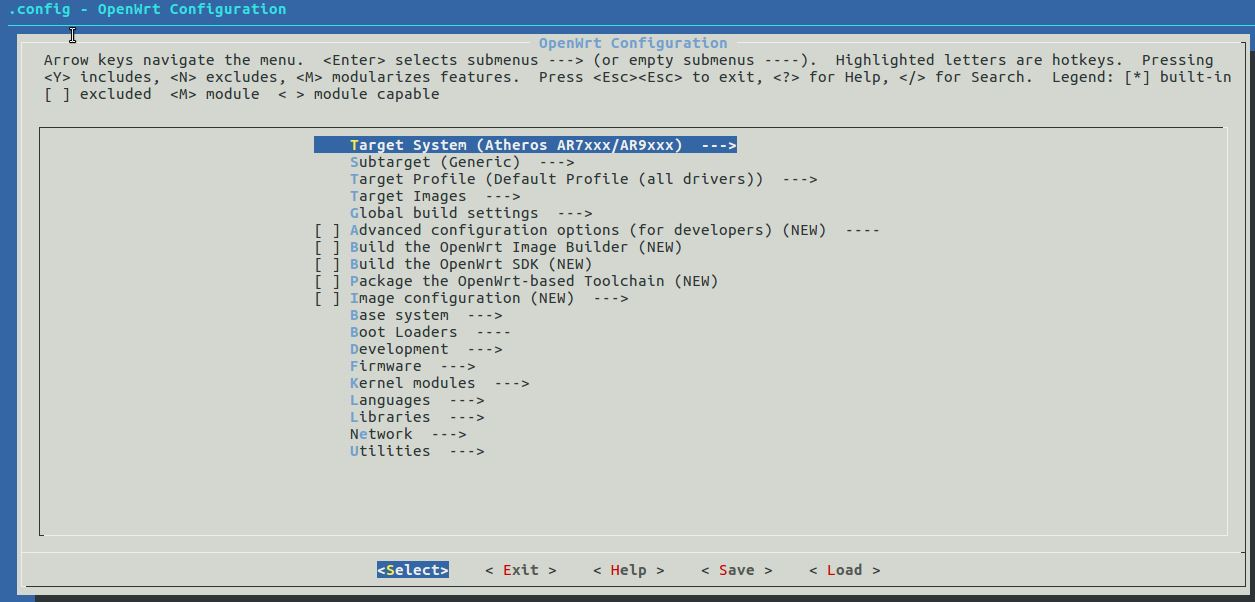
\includegraphics[width=\columnwidth]{image/menuconfig1.jpg}%
\caption{Menuconfig interface}%
\label{figure:menuconfig1}%-
\end{figure}

We are going to change a few things with this menu: the target system, the target profile, and the SDK.
First, we are going to put the target system to its right walue. In our case, we are using a GL-AR150. Therefore, we need to put:
\begin{lstlisting}[language=bash]
  'Atheros AR71xxx/AR9xxx'
\end{lstlisting}

If you are using a different router, you may have to choose another option.

Then, we are going to select GL-AR150 in the target profile.

Finally, we want to tick the box for 'Build the LEDE SDK' (or openwrt if your router is not using LEDE as an os).

We know save these changes and exit the menuconfig.

Now, we can finally build the SDK using the command:
\begin{lstlisting}[language=bash]
	###: make
\end{lstlisting}

This command may take a long time depending the power of your computer. For instance, on my Linux virtual machine (with 4GB of RAM and a laptop cpu) it took several hours to finish.

Once done, you will have a lot of new files. We are only interested in one repository:
\begin{lstlisting}[language=bash]
	staging_dir/toolchain-mips_24kc_gcc-5.4.0_musl-1.1.16
\end{lstlisting}

The name of the directory may change a bit but it will always start by toolchain.
So if you go to the 'bin' directory inside the toolchain, you should find the following file:
\begin{lstlisting}[language=bash]
	staging_dir/toolchain...bin/mips-openwrt-linux-musl-gcc
\end{lstlisting}

This executable is a c compiler for our router. We can use it on the linux computer to compile a c file. It will create an executable that can run on the router.


We know have our compiler. To use it we need to do the following steps:
\begin{itemize}
	\item export the bin directory in the PATH environment variable
	\item export a new environment variable called STAGING\_DIR (it will be used by the compiler
	\item precise to the makefile of the server where to find the compiler
\end{itemize}

Let's start by creating the environment variables. In your main repository, there is a file called .bashrc. This file is executed each time you start a shell. We are going to add two lines at the end of this file:
\begin{lstlisting}[language=bash]
	PATH=$PATH:~/staging_dir/toolchain.../bin/
	export STAGING_DIR=~/staging_dir/toolchain.../
\end{lstlisting}

Now we only need to slightly change the makefile. Go to the repository containing the sources.
In the makefile, there is at the top of the file a variable called SERVERCC.
This variable precise the compiler used for the server.c file.
To compile it for the router, we just need to change its value to the correct gcc: mips-openwrt-linux-musl-gcc
If we later want to compile the server.c file for the linux computer (to do some testing), we only need to change back this variable to gcc.


Now we can create the server exec file by doing:

\begin{lstlisting}[language=bash]
	###: make server
\end{lstlisting}

\large WARNING:\\
The server and the client have two mode DEBUG and normal. To change the mode of functioning, you have to change the value of a line in their respective c files. The line to change is:
\begin{lstlisting}[language=c]
	#define DEBUG 1
\end{lstlisting}
If the value of this line is 0, it means you are in DEBUG mode. Make sure to put any other number than 0 before doing make.

\subsubsection{Adding the server to the router}

We now have an executable called 'server'. In this part, we will:
\begin{itemize}
	\item add this file to the router
	\item automatize its start
\end{itemize}



To add the file to the router, we just use scp (which is a copy function over a ssh connection) to copy the executable anywhere in the router.


Now we are going to automatize the server. We want two things:
\begin{itemize}
	\item the server start during the boot
	\item if the server crash, a script is launching it again
\end{itemize}

First, let's start by writing the script that will start the server at the boot:


\begin{lstlisting}
#!/bin/sh /etc/rc.common

# The order you want these scripts to be run. 
# e.g Start=6 will run after scripts with Start=5 but before Start=7
START=6
STOP=12

# The command(s) you want to run on start
start() {        
        echo starting
	PATH_of_server_executable
}                 

# The command(s) you want to run on stop
stop() {          
        echo stopping
				
}
\end{lstlisting}



Now we want to restart the server if he crash.
To do achieve that, we are going to use crontab and the following script.

\begin{lstlisting}
	#!/bin/sh
	result=`netstat -an|grep 8800| grep LISTEN`
	if [ -z "$result" ]
	then
		/path_to_server
	fi
\end{lstlisting}



We will execute this script every 10 minutes.
By default cron is disable on lede. We can enable it with the following command:
\begin{lstlisting}
	/etd/init.d/cron enable
\end{lstlisting}

We can now run cron:
\begin{lstlisting}
	crontab -e
\end{lstlisting}


It will open a file with vi. On this file we want to add the following line
\begin{lstlisting}
*/10 * * * * path_to_script
\end{lstlisting}



If you want to adjust how often it repeat, here is how crontab work. The line is composed of the following elements
minute hour day(month) year day(week) command\_to\_execute

For the first 5 value, there are special characters:
\begin{itemize}
	\item * represents any value
	\item , is a value line separator
	\item / is used for step values
	\item - is a range of value
\end{itemize} 



\chapter{How to use it?}

Once the installation steps are done, using the client is quite easy.
You simply need to launch the client\_shell in a terminal using the command:
\begin{lstlisting}
	###: ./client_shell
\end{lstlisting}

It will launch a shell-like interface.
In this interface, you can input some commands to control the client.

We have two type of command:
\begin{itemize}
	\item built in functions: functions written in c to control the system
	\item classic shell command
\end{itemize}

We are mainly interested in the built in functions.
The available commands are:
\begin{itemize}
	\item help: list the available built in functions
	\item exit: close the client\_shell
	\item launch: launch a client
	\item findServers: update the list of available servers
	\item displayServers: display the available servers
	\item close: close a client
	\item list: list the clients currently running 
	\item log: start or stop logging the data for one client
\end{itemize}

If you type a function but do not put the right parameters, the shell will display a short message
explaining how to use the function properly.

Here is an example of process you want to do when starting the client\_shell for the first time:
First we want to find the available servers. So we type:
\begin{lstlisting}
	displayServers
\end{lstlisting}
We get a list of the available servers. Each server has a number in front of it. We can use this number to start a client who will communicate with this server.
\begin{lstlisting}
	launch 0
\end{lstlisting}

A new window pops up. This is the client we just created.
We can start another client on another server.
\begin{lstlisting}
	launch 1
\end{lstlisting}


Now we want to list the clients running. So we type:
\begin{lstlisting}
	list
\end{lstlisting}
We get a list of the clients running. Each client has a number in front of it. We can use this number to send messages to the client.


For instance, we may want to log the data of the first client in a file called "`Log;\_UHF"'.
\begin{lstlisting}
	log 0 Log_UHF
\end{lstlisting}
The client with the index 0 will start to log the data in the file Log\_UHF.

After a while, we think we have enough data and we want to stop logging them.
\begin{lstlisting}
	log 0 stop
\end{lstlisting}

With the same command log wa can stop it. However, it means stop can't be the filename.

Finally we want to shutdown all the clients.
\begin{lstlisting}
	close all
\end{lstlisting}
This will close all the clients and their connections. If we wanted to shutdown only one client, we just have to replace "`all"' by the number of the client.








\chapter{Unfinished parts}


\section{Wi-Fi monitoring}

I wanted to integrate some c code for this part but I unfortunately didn't have the time to do it. Right now, we have to use a temporary solution with the package tcpdump and wireshark (a graphic network tool to analyse messages going through the network).

tcpdump is a Linux package that can be installed on the routers. This package allow an user to scan all the messages going through an interface. Therefore, using this command, we can analyse the Wi-Fi communication going around the router.
We can install this package on the remote router.

Then on the computer in the lab, you simply have to use the following command:

\begin{lstlisting}[language=bash]
ssh root@192.168.8.11 tcpdump -i wlan0 -U -s0 -w - 'not port 22' | ... 
... sudo wireshark -k -i -
\end{lstlisting}

With this command, we launch the command tcpdump on the remote router. It will analyse the Wi-Fi interface called wlan0. Then the result of the tcpdump command is sent to our computer and displayed through wireshark. 



\section{Phone}


I managed to remotely control a phone using virtual machines. I had the phone plugged into one virtual machine, and I was controlling the phone in the other virtual machine.

All the component used for this solution were supposed to be available on the small routers. I was hoping it would work smoothly. However, when I tried it on the small routers it didn't work. I still have a proof of concept on virtual machines. It should be possible to make it work on the small router even if it needs to be a little tweaked.

The solution is based on:
\begin{itemize}
	\item adb (android debug bridge) and scrcpy on the computer
	\item usbip on the small router
\end{itemize}

scrcpy is a free open software that use adb to give the user a full control of his phone through a computer. When you launch scrcpy, it will reproduce the screen of your phone on the computer and you can use it.
There is only one issue with scrcpy. It is a very heavy software and can therefore not run on the small routers. 
The solution I came up with was to make scrcpy work on the computer. scrcpy will display the screen of your phone as long as adb can reach it. adb has two ways to reach a phone: through a usb connection or through the network. So I wanted to use the usb connection since the phone will be connected by Wi-Fi to the Mesh Extender and by usb to the remote router. On Linux, there is a package called usbip. This package can make a usb connection work over the network. So we have the phone connected to the remote router using usb. The router transfers this connection to the computer using the network. The computer can use scrcpy to control the phone.


\subsection{How to install scrcpy}


First, let's start by installing the required package:
\begin{lstlisting}
apt install ffmpeg libsdl2-2.0.0
apt install make gcc pkg-config meson libavcodec-dev 
	libavformat-dev libavutil-dev libsdl2-dev
apt install openjdk-8-jdk
\end{lstlisting}



Now we need to install android studio:
\begin{itemize}
	\item Download the compressed file on their website
  \item Extract the files
  \item Goto bin folder inside the extracted files
  \item Launch the studio.sh file: ./studio.sh
  \item It will open the installer, follow the instruction
\end{itemize}


Activate sdk licenses:
\begin{itemize}
	\item Go to ~/Android/Sdk/tools/bin
	\item ./sdkmanager --licenses
\end{itemize}
        

Create the Android SDK environment variable:
\begin{lstlisting}
export ANDROID_HOME=~/Android/Sdk
\end{lstlisting}

Watch out, the path could be ~/android/sdk instead of ~/Android/Sdk	.


Clone and install scrcpy:
\begin{lstlisting}
...:# git clone https://github.com/Genymobile/scrcpy



...:# cd scrcpy/
...:scrcpy# mkdir x
...:scrcpy# meson x --buildtype release --strip -Db_lto=true
The Meson build system
Version: 0.45.1
Source dir: .../scrcpy
Build dir: .../scrcpy/x
Build type: native build
Project name: scrcpy
Native C compiler: cc (...)
Build machine cpu family: x86_64
Build machine cpu: x86_64
Found pkg-config: /usr/bin/pkg-config (0.29.1)
Native dependency libavformat found: YES 57.83.100
Native dependency libavcodec found: YES 57.107.100
Native dependency libavutil found: YES 55.78.100
Native dependency sdl2 found: YES 2.0.8
Configuring config.h using configuration
Program ./scripts/build-wrapper.sh found: YES (...)
Build targets in project: 6
Found ninja-1.8.2 at /usr/bin/ninja
\end{lstlisting}			
				
				


 \chapter{Resources used}

In this part, you will find every useful references I used to create the test network. If you want to have a better understanding on the functioning of the solution, you can take a look at them

\section{Network}
Source for relayd: \url{https://wiki.openwrt.org/doc/recipes/relayclient}

DNS and DHCP: \url{https://wiki.openwrt.org/doc/uci/dhcp}

\section{server}


function poll: \url{https://www.ibm.com/support/knowledgecenter/en/ssw\_i5\_54/rzab6/poll.htm}

cross-compilation: \url{https://manoftoday.wordpress.com/2007/10/11/writing-and-compiling-a-simple-program-for-openwrt/}
cross-compilation: \url{https://github.com/airplug/airplug/wiki/Cross-compiling-for-OpenWRT}


\section{client}

signal handling: \url{https://stackoverflow.com/questions/5546223/signals-received-by-bash-when-terminal-is-closed}


\section{client\_shell}

tutorial to write a shell in C: \url{https://brennan.io/2015/01/16/write-a-shell-in-c/}
customise xterm: \url{https://scarygliders.net/2011/12/01/customize-xterm-the-original-and-best-terminal/}



\section{Phone}

usb over ip: \url{https://wiki.openwrt.org/doc/howto/usb.iptunnel}
scrcpy: \url{https://github.com/Genymobile/scrcpy}
FIFO: \url{https://www.tldp.org/LDP/lpg/node11.html}



\section{Other useful references}
Boot structure of openwrt: \url{https://medium.com/openwrt-iot/lede-openwrt-boot-structure-e689c4ddea91}
Scheduling tasks with cron on openwrt: \url{https://medium.com/openwrt-iot/openwrt-scheduling-tasks-6e19d507ae45}
%\chapter{How it works?}

In this part, you will find an explanation of every program used in this project:
\begin{itemize}
	\item the server.c
	\item the client.c
	\item the client\_shell.c
\end{itemize}


\section{server.c}



\section{client\_shell.c}


\section{client.c}









%%%%%%%%%%%%%%%%%%%%%%%%%%%%%%%%%%%%%%%%%%%%%%%%%%%%%%%%%%%%%
%% BIBLIOGRAPHY AND OTHER LISTS
%%%%%%%%%%%%%%%%%%%%%%%%%%%%%%%%%%%%%%%%%%%%%%%%%%%%%%%%%%%%%
%% A small distance to the other stuff in the table of contents (toc)
\addtocontents{toc}{\protect\vspace*{\baselineskip}}

%% The Bibliography
%% ==> You need a file 'literature.bib' for this.
%% ==> You need to run BibTeX for this (Project | Properties... | Uses BibTeX)
%\addcontentsline{toc}{chapter}{Bibliography} %'Bibliography' into toc
%\nocite{*} %Even non-cited BibTeX-Entries will be shown.
%\bibliographystyle{alpha} %Style of Bibliography: plain / apalike / amsalpha / ...
%\bibliography{literature} %You need a file 'literature.bib' for this.

%% The List of Figures
\clearpage
\addcontentsline{toc}{chapter}{List of Figures}
\listoffigures

%% The List of Tables



%%%%%%%%%%%%%%%%%%%%%%%%%%%%%%%%%%%%%%%%%%%%%%%%%%%%%%%%%%%%%
%% APPENDICES
%%%%%%%%%%%%%%%%%%%%%%%%%%%%%%%%%%%%%%%%%%%%%%%%%%%%%%%%%%%%%
\appendix
%% ==> Write your text here or include other files.

%\input{FileName} %You need a file 'FileName.tex' for this.


\end{document}

